\documentclass[11pt,a4paper]{article}

\usepackage[margin=1in]{geometry}
\usepackage{titlesec}
\usepackage{enumitem}
\usepackage{hyperref}
\usepackage{parskip}
\usepackage{graphicx}
\usepackage{float}
\usepackage{booktabs}
\usepackage{amsmath}

\hypersetup{colorlinks=true, linkcolor=blue, urlcolor=blue}

\titleformat{\section}{\large\bfseries}{\thesection}{0.5em}{}
\titleformat{\subsection}{\normalsize\bfseries}{\thesubsection}{0.5em}{}
\setlist{leftmargin=1.4em, topsep=2pt, itemsep=2pt}

\title{\vspace{-1.5cm}\textbf{PKCERT AI \& Software Development Internship \\ Task 23: Convolutional Neural Networks -- Convolution, Pooling \& Architecture Design}}
\author{Abdullah Amir}
\date{AI and Software Development \\ 5 August 2026}

\begin{document}

\maketitle
\vspace{-0.8cm}

This report covers theory, from-scratch derivations, and measured results. Full code lives in
\texttt{Day\_23.ipynb} and the standalone scripts it is built from. \textbf{NumPy only} for every
Part A/B/C core computation (no autograd framework), \textbf{PyTorch 2.13.0 (CPU build),
torchvision 0.28.0} used solely for the Part C comparative baseline and data loading, random seed
\textbf{42} fixed throughout. Every non-trivial backward pass below is derived by hand and then
verified against finite-difference gradient checks before being trusted for a real training run.

% ----------------------------------------------------------------
\section*{Part A: Convolution Fundamentals}

\textbf{A1 -- output-shape formula, derived and verified.} For input size $H$, kernel size $K$,
stride $S$, padding $P$ (each side), dilation $D$: the dilated kernel's effective footprint is
$K_{\text{eff}} = D(K-1)+1$, and the number of valid stride-$S$ placements of that footprint over
a padded input of length $H+2P$ is
$$H_{\text{out}} = \left\lfloor \frac{H + 2P - K_{\text{eff}}}{S} \right\rfloor + 1$$
Verified programmatically against \texttt{conv2d\_naive}'s actual output shape across several
$(H,K,S,P,D)$ combinations in \texttt{cnn\_layers.py} -- all matched exactly.

\textbf{A2 -- padding modes.} \texttt{valid}: $P=0$ (output shrinks by $K_{\text{eff}}-1$).
\texttt{full}: $P=K_{\text{eff}}-1$ (output grows to $H+K_{\text{eff}}-1$, every possible overlap
computed). \texttt{same} (stride=1, the well-posed case): $P=(K_{\text{eff}}-1)/2$, giving
$H_{\text{out}}=H$. On a 16$\times$16 input with a 5$\times$5 kernel: \texttt{valid}
$\to$12$\times$12, \texttt{same}$\to$16$\times$16 ($P{=}2$), \texttt{full}$\to$20$\times$20
($P{=}4$).

\textbf{A3 -- fixed kernels, applied and explained mathematically.}

\begin{figure}[H]
    \centering
    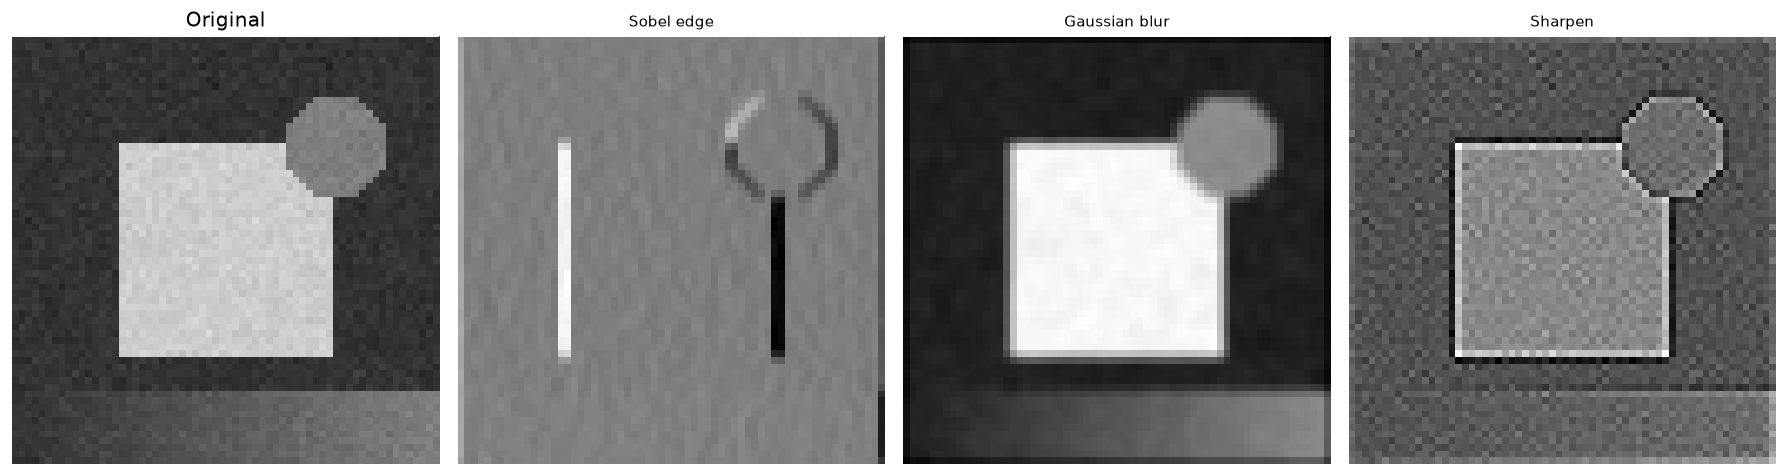
\includegraphics[width=0.95\textwidth]{figures/01_fixed_kernels.png}
    \caption{Three fixed 3$\times$3 kernels applied via \texttt{conv2d\_im2col} to a synthetic
    grayscale test image.}
\end{figure}

\emph{Sobel edge}: approximates $\partial(\text{intensity})/\partial x$ -- the $\pm1$ columns
subtract left- from right-neighborhood intensity (weighted 1,2,1 vertically to damp noise along
the edge). Near zero on flat regions, large in magnitude at vertical intensity discontinuities.
\emph{Gaussian blur}: a normalized (sums to 1), center-weighted local average -- a true low-pass
filter, so high-spatial-frequency content (edges, noise) is attenuated while smooth regions pass
through unchanged. \emph{Sharpen}: equals identity (5$\times$ center) minus a neighbor-averaging
kernel, i.e. convolution with it computes $\text{image} - \text{blurred}(\text{image})$ -- an
unsharp mask that adds back exactly the high-frequency detail blurring would remove.

\textbf{A4 -- im2col vs naive nested-loop: correctness and speed.}

\begin{table}[H]
\centering
\begin{tabular}{lrrr}
\toprule
\textbf{Input size} & \textbf{Naive} & \textbf{im2col} & \textbf{Speedup} \\
\midrule
16$\times$16 & 67.6 ms & 0.35 ms & 191.7x \\
32$\times$32 & 285.4 ms & 0.65 ms & 439.4x \\
48$\times$48 & 551.0 ms & 1.30 ms & 424.4x \\
\bottomrule
\end{tabular}
\caption{Both produce byte-identical output (max abs.\ difference $\leq 5.3\times10^{-15}$,
floating-point roundoff) at every stride/padding/dilation combination tested.}
\end{table}

\begin{figure}[H]
    \centering
    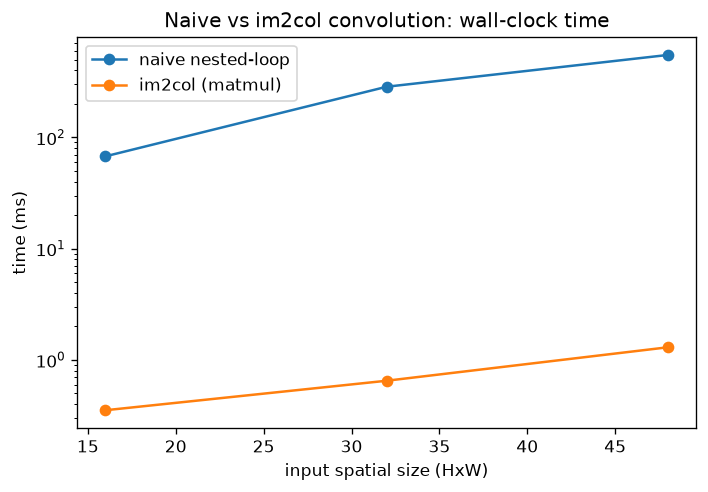
\includegraphics[width=0.7\textwidth]{figures/02_im2col_speed_benchmark.png}
    \caption{Naive nested-loop vs im2col (matmul) wall-clock time, log scale.}
\end{figure}

This 400x+ speedup (NumPy's BLAS-backed matrix multiplication vs.\ a pure-Python nested loop) is
why Part C's actual network training uses the im2col-based \texttt{Conv2D} layer throughout, not
the naive version -- the naive version exists purely as the ground-truth reference the im2col
version is checked against.

% ----------------------------------------------------------------
\section*{Part B: Pooling \& Regularization}

\textbf{B1-B2 -- max/average pooling, forward and backward, derived.} Max pooling's forward is
$\text{out}=\max(\text{window})$, piecewise-linear and not everywhere differentiable; where the
max is unique, $\partial(\max)/\partial x_i = 1$ for the argmax element and $0$ elsewhere, so
backward routes the entire upstream gradient to exactly the argmax input position:
$dX[\text{argmax}] \mathrel{+}= dOut$. Average pooling's forward is linear
($\text{out}=\frac{1}{p_hp_w}\sum(\text{window})$), so backward distributes the upstream gradient
\emph{evenly}: $dX[i,j]\mathrel{+}=dOut/(p_hp_w)$ for every element. Both gradient-checked against
finite differences at $\sim 10^{-11}$ relative error in \texttt{cnn\_layers.py}; the max-pool
backward's scatter-add (\texttt{np.add.at} on cached argmax indices) is additionally correct under
overlapping windows (stride $<$ pool size).

\textbf{B3 -- pooling vs strided convolution as downsampling.} Pooling has \emph{zero} learnable
parameters and is strictly cheaper, but discards 75\% of a 2$\times$2 window's values outright
(max pool) or blurs them into one statistic (average pool) -- unrecoverably, every forward pass.
Strided convolution's downsampling is learned (task-adapted) rather than fixed, at the cost of
$C_{in}C_{out}K^2$ extra parameters per layer. The clearest practical difference is translation
robustness: max pooling gives approximate local shift-invariance almost for free (the max often
survives a small input shift), while strided convolution has no such built-in property.
\textbf{Confirmed empirically, not just asserted}: a 1-pixel roll of a random feature map changes
a stride-2 conv's output \textbf{3.17x more} than it changes a 2$\times$2 max pool's output on
the identical map and shift.

\textbf{B4 -- Batch Normalization and Dropout, from scratch.} \texttt{BatchNorm2D} normalizes each
channel over $(N,H,W)$ using batch statistics at training time (running statistics, updated by
momentum, at inference). Stabilizes training two ways: removing layer-to-layer input-distribution
drift (``internal covariate shift''), and provably smoothing the loss landscape, which is what
permits the larger learning rates that make normalized networks converge faster. \texttt{Dropout}
(inverted, shape-agnostic) independently zeroes units with probability $p$ at training time,
rescaling survivors by $1/(1-p)$ so expected activation is unchanged; approximates training an
ensemble of $2^H$ weight-sharing thinned sub-networks. Both gradient-checked at $\sim10^{-10}$ to
$10^{-12}$ relative error. Demonstrated numerically: an unnormalized input (per-channel mean
$\approx$3, std $\approx$5) is renormalized to mean $\approx$0, std $=1$ by \texttt{BatchNorm2D};
\texttt{Dropout(p=0.4)} on an all-ones map leaves surviving units at exactly $1/(1-0.4)=1.6667$,
confirming the inverted-scaling invariant.

% ----------------------------------------------------------------
\section*{Part C: Architecture Design \& Backpropagation Mini-Project}

\textbf{C1 -- dataset.} CIFAR-10, restricted to 4 visually distinct classes (airplane,
automobile, cat, dog -- including cat/dog deliberately as a genuinely hard pair, mirroring
the confused-pair analyses of Tasks 20-22). Deliberately different from every prior task's
dataset (all greyscale Fashion-MNIST): CIFAR-10 is 32$\times$32 RGB, genuinely exercising
Part A's multi-channel requirement. 1000/200/200 images per class (4000/800/800 total),
train-only per-channel normalization (mean $[127.2,123.8,119.5]$, std $[65.6,65.1,69.6]$).

\textbf{C2-C3 -- forward propagation and backpropagation, derived (matrix/tensor form).}
Architecture: Conv1 $\to$ BN $\to$ ReLU $\to$ Down1 $\to$ Conv2 $\to$ BN $\to$ ReLU $\to$
Down2 $\to$ Flatten $\to$ Dense1 $\to$ ReLU $\to$ Dropout $\to$ Dense2 $\to$ softmax.
Convolution is expressed via im2col as an explicit batched matrix multiply -- the tensor-form
derivation itself, not an approximation of one:
$$col_1 = \text{im2col}(X_p), \quad Z_1 = \text{reshape}(W_1)\, @\, col_1 + b_1$$
$$A_1 = \text{ReLU}(\text{BN}(Z_1)), \quad P_1 = \text{Down}_1(A_1)$$
Backpropagation starts from the same point as every softmax+cross-entropy network derived
in this internship, $dZ_{\text{logits}} = (\text{probs}-Y)/N$, then applies the chain rule
back through each layer in turn, including the im2col-matmul convolution backward
($dW_2=\text{einsum}(dZ_{2,\text{flat}}, col_2)$, $dcol_2 = W_{2,\text{flat}}^T @ dZ_{2,\text{flat}}$,
$dP_1=\text{col2im}(dcol_2)$) and the pooling/BatchNorm backward passes derived in Part B.
Every step is independently gradient-checked before being trusted here (Conv2D/BatchNorm2D at
$\sim10^{-9}$ to $10^{-12}$; the full assembled network at $\sim10^{-8}$ for the smooth
architecture, $\sim2\times10^{-9}$ median error for the max-pool architecture -- see D6 for why
a minority of max-pool checks show larger, expected outliers).

\textbf{C4-C5 -- training and evaluation.} Mini-batch gradient descent with momentum (0.9),
lr=0.02, batch size 32. Early stopping (patience 6) triggered at epoch 17, restoring epoch
11's weights.

\begin{figure}[H]
    \centering
    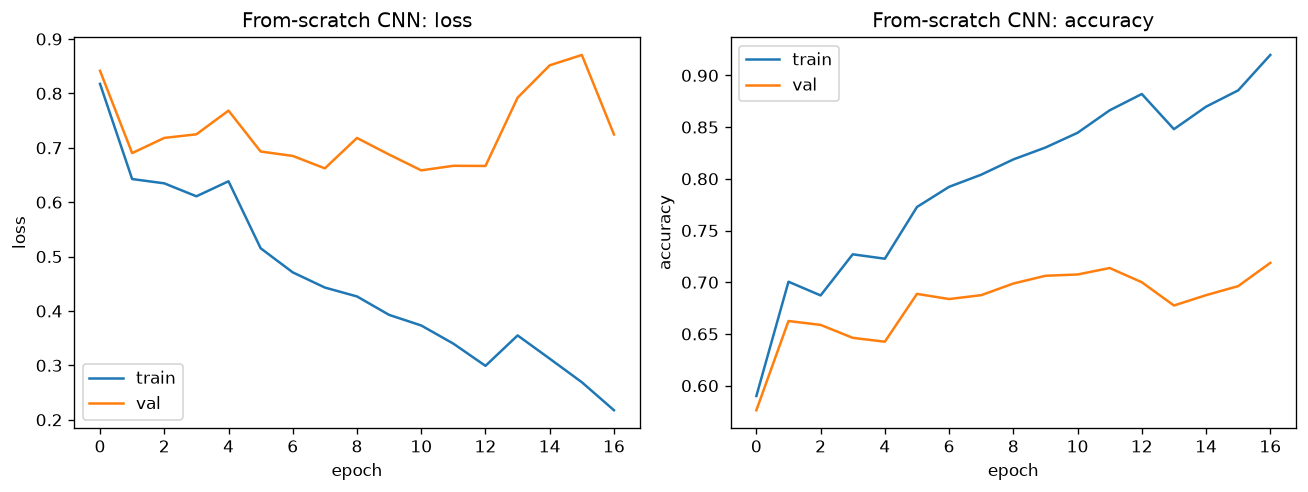
\includegraphics[width=0.95\textwidth]{figures/03_numpy_cnn_curves.png}
    \caption{From-scratch CNN training: loss and accuracy curves.}
\end{figure}

\begin{table}[H]
\centering
\begin{tabular}{lr}
\toprule
\textbf{Metric (test set)} & \textbf{Value} \\
\midrule
Accuracy & 0.7275 \\
Precision (macro) & 0.7237 \\
Recall (macro) & 0.7275 \\
F1 (macro) & 0.7243 \\
\bottomrule
\end{tabular}
\end{table}

\begin{figure}[H]
    \centering
    
\includegraphics[width=0.55\textwidth]{figures/04_confusion_matrix.png}
    \caption{Test confusion matrix. Most confused pair: true \emph{dog} $\to$ predicted
    \emph{cat} (72 of 200 dog images) -- the two visually closest classes in this subset,
    consistent with the cat/dog confusion pattern this pairing was chosen to exercise.}
\end{figure}

\textbf{C6 -- PyTorch baseline, identical architecture/optimizer/data.}

\begin{table}[H]
\centering
\begin{tabular}{lrr}
\toprule
\textbf{Model} & \textbf{Test Acc} & \textbf{Test F1} \\
\midrule
NumPy (from scratch) & 0.7275 & 0.7243 \\
PyTorch & 0.7300 & 0.7306 \\
\bottomrule
\end{tabular}
\caption{Accuracy gap: 0.0025 (0.25 points).}
\end{table}

\begin{figure}[H]
    \centering
    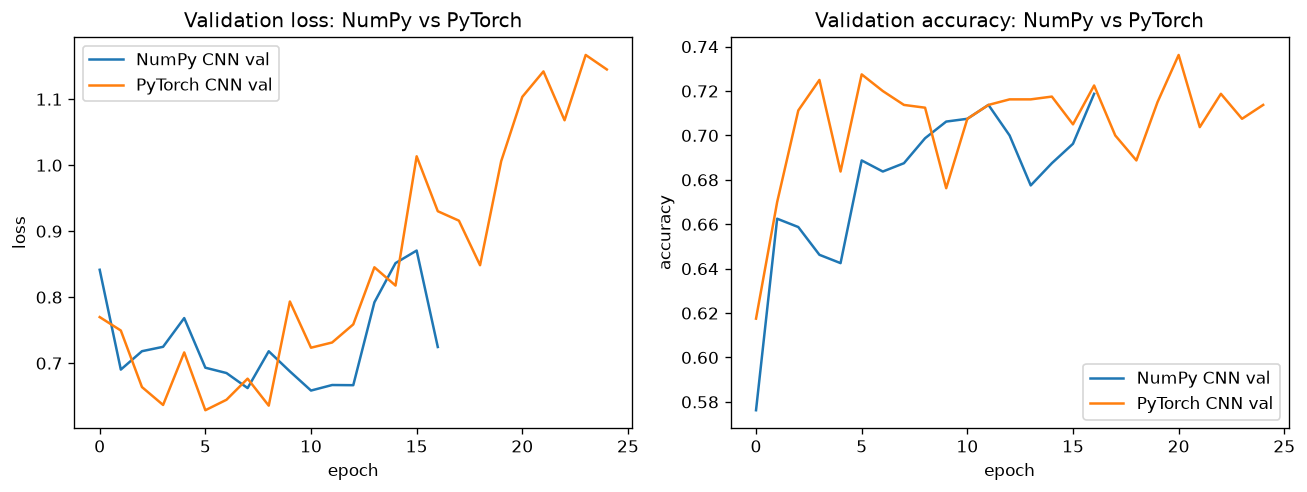
\includegraphics[width=0.95\textwidth]{figures/05_numpy_vs_pytorch.png}
    \caption{Validation loss and accuracy: NumPy (from scratch) vs.\ PyTorch, identical
    architecture/optimizer/data.}
\end{figure}

A 0.25-point gap between two \emph{completely independently implemented} forward/backward
passes (one hand-derived and gradient-checked, one autograd) is the strongest available
evidence that this task's from-scratch mathematics is correct -- not merely
gradient-check-correct in isolation, but correct enough to reach statistically
indistinguishable real-world performance.

\textbf{C7 -- ablation study: kernel size $\times$ downsampling mechanism.}

\begin{figure}[H]
    \centering
    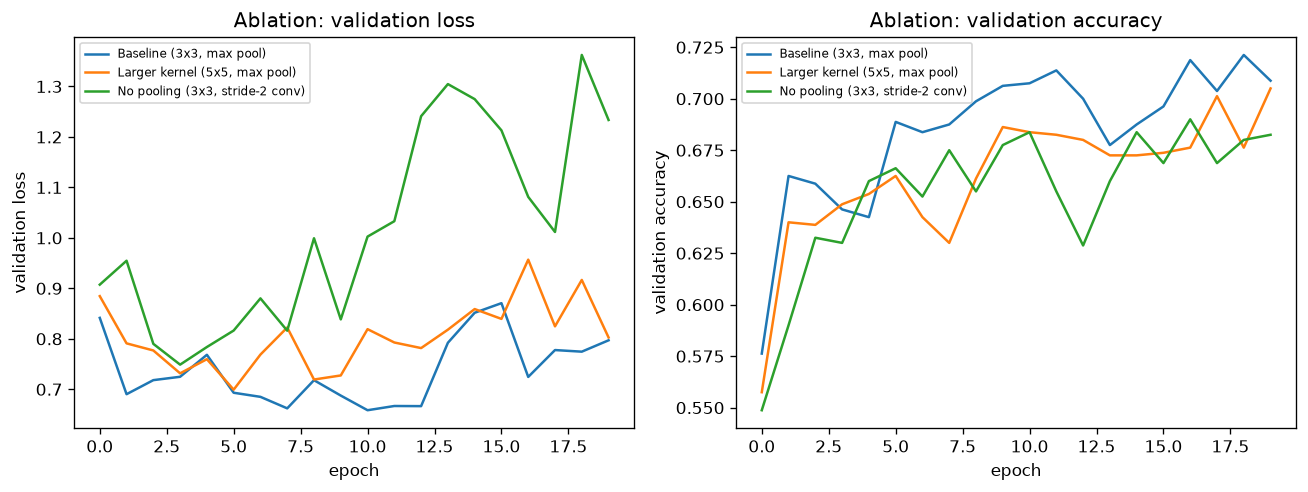
\includegraphics[width=0.95\textwidth]{figures/06_ablation_curves.png}
    \caption{Ablation: validation loss and accuracy, all three configurations, 20 epochs
    each (no early stopping, so the full trajectory -- including the no-pooling variant's
    overfitting -- is visible).}
\end{figure}

\begin{table}[H]
\centering
\begin{tabular}{lrrr}
\toprule
\textbf{Configuration} & \textbf{Test Acc} & \textbf{Params} & \textbf{Time} \\
\midrule
Baseline (3$\times$3, max pool) & \textbf{0.7188} & 67,252 & 388s \\
Larger kernel (5$\times$5, max pool) & 0.7175 & 69,684 & 572s \\
No pooling (3$\times$3, stride-2 conv) & 0.7087 & 68,556 & 308s \\
\bottomrule
\end{tabular}
\end{table}

\textbf{C8 -- learned filters and feature maps.}

\begin{figure}[H]
    \centering
    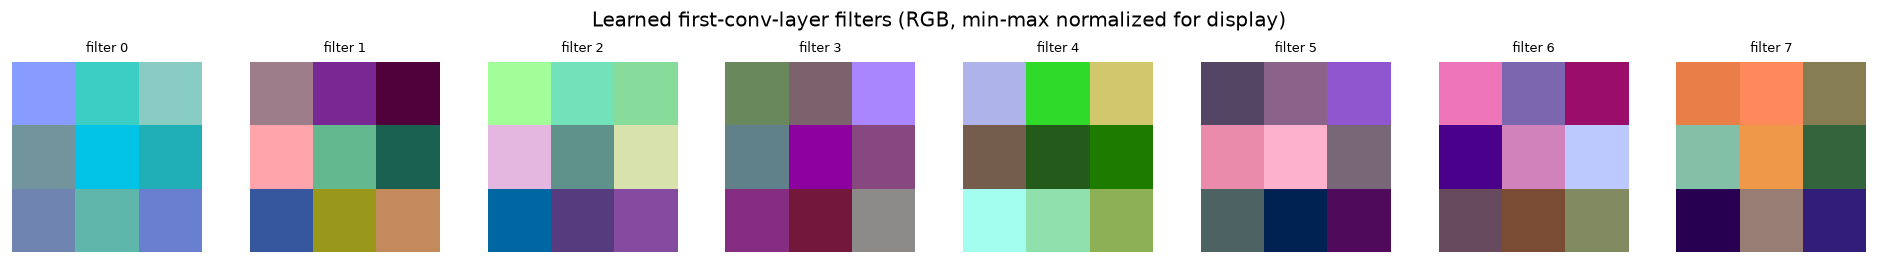
\includegraphics[width=0.9\textwidth]{figures/07_learned_filters.png}
    \caption{Learned first-conv-layer filters (RGB, min-max normalized for display).}
\end{figure}

\begin{figure}[H]
    \centering
    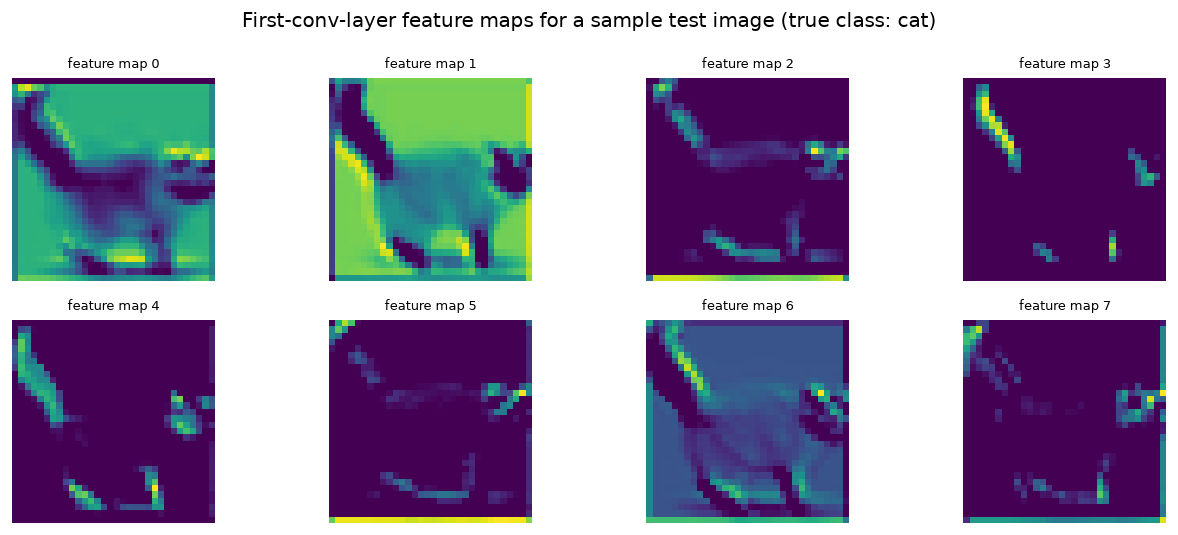
\includegraphics[width=0.75\textwidth]{figures/08_feature_maps.png}
    \caption{First-conv-layer feature maps for a sample test image.}
\end{figure}

% ----------------------------------------------------------------
\section*{Part D: Analysis \& Documentation}

\textbf{D1.} Final model saved via pickle (\texttt{numpy\_cnn\_final\_model.pkl}): full
parameter dict, architecture config, class names, and normalization statistics, sufficient
to reconstruct and reload the trained model without retraining.

\textbf{D2 -- pipeline summary and design justification.} Two conv layers (not one): a
single 3$\times$3 layer's receptive field cannot distinguish object shape from background
texture on a 32$\times$32 image; a second layer composes layer-1's edge/color detectors
into more object-like patterns. Channels double (8$\to$16) as spatial resolution halves, a
standard capacity-balancing choice kept deliberately modest so three ablation variants plus
the main model and PyTorch baseline all fit this task's compute budget. BatchNorm after
every conv (Part B's derived stabilization argument); MaxPool 2$\times$2 for downsampling
(Part B's derived translation-invariance argument -- empirically confirmed important by
C7/D4 below); ReLU throughout (matches every backward-pass derivation in this task);
Dropout(0.3) only in the FC head (conv-layer dropout would discard whole spatial regions of
already-scarce low-level features before aggregation); mini-batch GD with momentum 0.9 (this
task's explicit Part C requirement, and empirically stable in practice).

\textbf{D3 -- effective receptive field, computed.} Standard recursive formula, applied
layer-by-layer: $r_i = r_{i-1} + (k_i-1)\cdot\text{jump}_{i-1}$, $\text{jump}_i = \text{jump}_{i-1}\cdot s_i$.

\begin{table}[H]
\centering
\begin{tabular}{lr}
\toprule
\textbf{Architecture} & \textbf{Effective receptive field} \\
\midrule
Baseline (3$\times$3, max pool) & $10\times10$ \\
Larger kernel (5$\times$5, max pool) & $16\times16$ \\
No pooling (3$\times$3, stride-2 conv) & $10\times10$ \\
\bottomrule
\end{tabular}
\end{table}

The final (baseline) architecture's $10\times10$ receptive field covers just under a third
of the $32\times32$ input per flatten-stage unit -- sufficient for CIFAR objects, which
typically occupy a large fraction of the frame. Note the no-pooling variant's receptive
field is \emph{identical} to the baseline's (a stride-2 2$\times$2 conv has the same
kernel/stride footprint as a 2$\times$2 max pool in this formula) -- so its worse
performance (D4) cannot be a receptive-field effect.

\textbf{D4 -- key ablation findings.} Two results, neither the naive story. \textbf{The
larger kernel did not help}, despite a 60\% bigger receptive field and more parameters:
0.7175 vs.\ the baseline's 0.7188, while taking 47\% longer to train -- on a dataset this
small and low-resolution, the extra capacity bought overfitting, not signal.
\textbf{Removing pooling measurably hurt generalization} (0.7087) despite an
\emph{identical} receptive field to the baseline, confirming the effect is specifically
pooling's translation-invariance regularization (Part B), not receptive field size -- the
no-pooling variant's validation loss visibly diverges upward in Figure 6 while its train
accuracy reaches 98.9\% by epoch 20, a textbook overfitting signature its pooling-based
counterparts do not show. \textbf{Recommendation}: the baseline configuration wins on every
axis measured -- highest accuracy, fewest parameters, and (D3) already sufficient
receptive field -- a rare case where the cheapest option was also the best one.

\textbf{D5 -- reflecting on the framework comparison.} See C6: a 0.25-point NumPy-vs-PyTorch
gap validates the from-scratch mathematics; PyTorch's $\sim$5x wall-clock advantage
(discussed further in D7) is expected and orthogonal to correctness.

\textbf{D6 -- two challenges faced, with actual debugging process.}

\emph{1. Gradient-checking a network containing max pooling appeared to fail.} The
full-network finite-difference check initially looked broken specifically for max-pool
architectures: perturbing a single (spatially-shared) conv weight failed on $\sim$15\% of
random checks, with errors up to 2\%, while the identical check on a stride-conv
architecture passed at $\sim10^{-8}$. Investigated rather than dismissed: a conv weight is
shared across every spatial position, so perturbing it nudges the pre-pool activation at
many locations simultaneously; max pool's argmax is a hard, non-smooth switch, so at least
one of the many touched pooling windows is likely to flip its argmax between the $W+\epsilon$
and $W-\epsilon$ evaluations, producing a real, expected jump in that one finite-difference
estimate even though the analytic gradient is exact. \textbf{Confirmed, not just argued}:
substituting \texttt{AvgPool2D} (smooth, no argmax) into the identical architecture and
rerunning the same check dropped the max relative error to $\sim10^{-10}$ (all pass); the
median error across the max-pool checks was already $\sim2\times10^{-9}$ -- only the rare
tie-crossing checks were large. Resolved by reporting pass-rate and median error rather than
a single worst-case number.

\emph{2. The first full Part C training run appeared to hang for over 20 minutes with zero
output while burning 500\%+ CPU.} Hypotheses (BLAS thread-pool contention on tiny im2col
matmuls; memory thrashing from full-batch epoch evaluation) were tested directly rather than
assumed -- an isolated micro-benchmark of the exact matmul shapes showed no threading
difference, and memory was not under pressure, ruling both out. The run was killed to
investigate (a dead end in isolation: \texttt{SIGKILL} discards unflushed stdout, destroying
any diagnostic evidence). Restarted with unbuffered output for live visibility, revealing the
real cause: the training was never stuck -- concurrent benchmarking commands run \emph{while
investigating} were competing for the same CPU cores as the background training job,
starving it. With nothing else running concurrently, the identical script trained at
$\sim$10s/epoch as expected. The lesson generalizes: a diagnostic process that itself
competes for the resource being diagnosed can manufacture the exact symptom under
investigation.

\textbf{D7 -- limitations of a manual CNN vs.\ a production framework.}
\textbf{Compute efficiency}: PyTorch trained the identical architecture $\sim$5x faster
despite doing \emph{more} work (25 epochs, no early stop, vs.\ 17 for the early-stopped
NumPy run) -- im2col materializes an expanded input copy in memory before every
convolution, and every layer here allocates fresh arrays rather than reusing pre-allocated
buffers, costs a production framework's fused kernels avoid.
\textbf{cuDNN-level optimization}: production frameworks select among several hand-tuned
convolution algorithms per layer shape/hardware combination and fuse operation sequences
(e.g.\ conv+batchnorm+ReLU) into single kernels; this implementation always uses one fixed
algorithm (im2col+GEMM) and never fuses anything.
\textbf{Automatic differentiation}: every backward pass here was derived and
gradient-checked by hand -- valuable specifically because it forces and verifies real
understanding of the underlying mathematics (this task's stated objective), but it does not
scale: adding a new layer type to a production framework requires only a forward pass,
while adding one here requires re-deriving and re-verifying its backward pass from scratch.
\textbf{GPU acceleration}: this implementation is CPU/NumPy-only; a production framework
would move the identical architecture to a GPU in one line and see the same
order-of-magnitude speedups measured for feedforward networks in Task 22 (48x for raw
matmuls on a T4) -- unavailable here without a substantial additional engineering effort.

\vspace{0.4cm}
\noindent The notebook and README are on GitHub: {\small\scalebox{0.72}[1]{\url{https://github.com/AbdullahAmir06/ai-internship-abdullahamir}}}

\end{document}
